% ------------------------------------------------------------------
\documentclass[12 pt]{article} % A4 paper set by geometry package below
\pagenumbering{arabic}
\setlength{\parindent}{10 mm}
\setlength{\parskip}{12 pt}

% Nimbus Sans font should be reasonably legible
\usepackage{helvet}
\renewcommand{\familydefault}{\sfdefault}
\usepackage[T1]{fontenc}  % Without this \textsterling produces $

% Section header spacing
\usepackage{titlesec}
\titlespacing\section{0pt}{12pt plus 4pt minus 2pt}{0pt plus 2pt minus 2pt}
\titlespacing\subsection{0pt}{12pt plus 4pt minus 2pt}{0pt plus 2pt minus 2pt}
\titlespacing\subsubsection{0pt}{12pt plus 4pt minus 2pt}{0pt plus 2pt minus 2pt}

\usepackage{amsmath}
\usepackage{amssymb}
\usepackage{graphicx}
\usepackage{verbatim}    % For comment
\usepackage[paper=a4paper, marginparwidth=0 cm, marginparsep=0 cm, margin=2.5 cm, includemp]{geometry}
\usepackage[pdftex, pdfstartview={FitH}, pdfnewwindow=true, colorlinks=true, citecolor=blue, filecolor=blue, linkcolor=blue, urlcolor=blue, pdfpagemode=UseNone]{hyperref}

% Put module code and last-modified date in footer
\usepackage{fancyhdr}
\pagestyle{fancy}
\fancyhf{}
\renewcommand{\headrulewidth}{0pt}
\cfoot{{\small \thisunit}\hfill \thepage\hfill {\small \moddate}}

% Hopefully address Canvas complaints about pdf tagging
%\usepackage[tagged]{accessibility}
\hypersetup {
  pdfauthor={David Schaich},
  pdftitle={StatMech Tutorial},
}
% ------------------------------------------------------------------



% ------------------------------------------------------------------
% Shortcuts
\newcommand{\be}{\ensuremath{\beta} }
\newcommand{\eps}{\ensuremath{\varepsilon} }
\newcommand{\om}{\ensuremath{\omega} }
\newcommand{\vev}[1]{\ensuremath{\left\langle #1 \right\rangle} }
\newcommand{\pderiv}[2]{\ensuremath{\frac{\partial #1}{\partial #2}} }
% ------------------------------------------------------------------



% ------------------------------------------------------------------
\begin{document}
\newcommand{\thisunit}{MATH327 Tutorial (Solid)}
\newcommand{\moddate}{Last modified 20 Mar.~2025}
\begin{center}
  {\Large \textbf{MATH327: StatMech and Thermo, Spring 2025}} \\[12 pt]
  {\Large \textbf{Tutorial exercises \ --- \ Einstein solid}} \\[24 pt]
\end{center}

These exercises will be introduced in our 20 March tutorial, and you'll have the week until our next tutorial on 27 March to work on them.
They explore another example in which a system with quantized energies is analysed in a classical way (employing the micro-canonical and canonical ensembles).

Our goal is to model the experimental heat capacity data points for several solids in the figure below (from Schroeder's \textit{Introduction to Thermal Physics}).\footnote{Experimentally it is easier to measure the heat capacity at constant \textit{pressure}, $c_p$, rather than at constant volume, but the difference between $c_p$ and $c_v$ is negligible for our purposes here.}
The heat capacities for all three solids have the same qualitative features --- approaching zero as $T \to 0$ (one way of expressing the \href{https://en.wikipedia.org/wiki/Third_law_of_thermodynamics#Specific_heat}{third law of thermodynamics}) and increasing towards a roughly constant value at higher temperatures. \\[-24 pt]
\begin{center}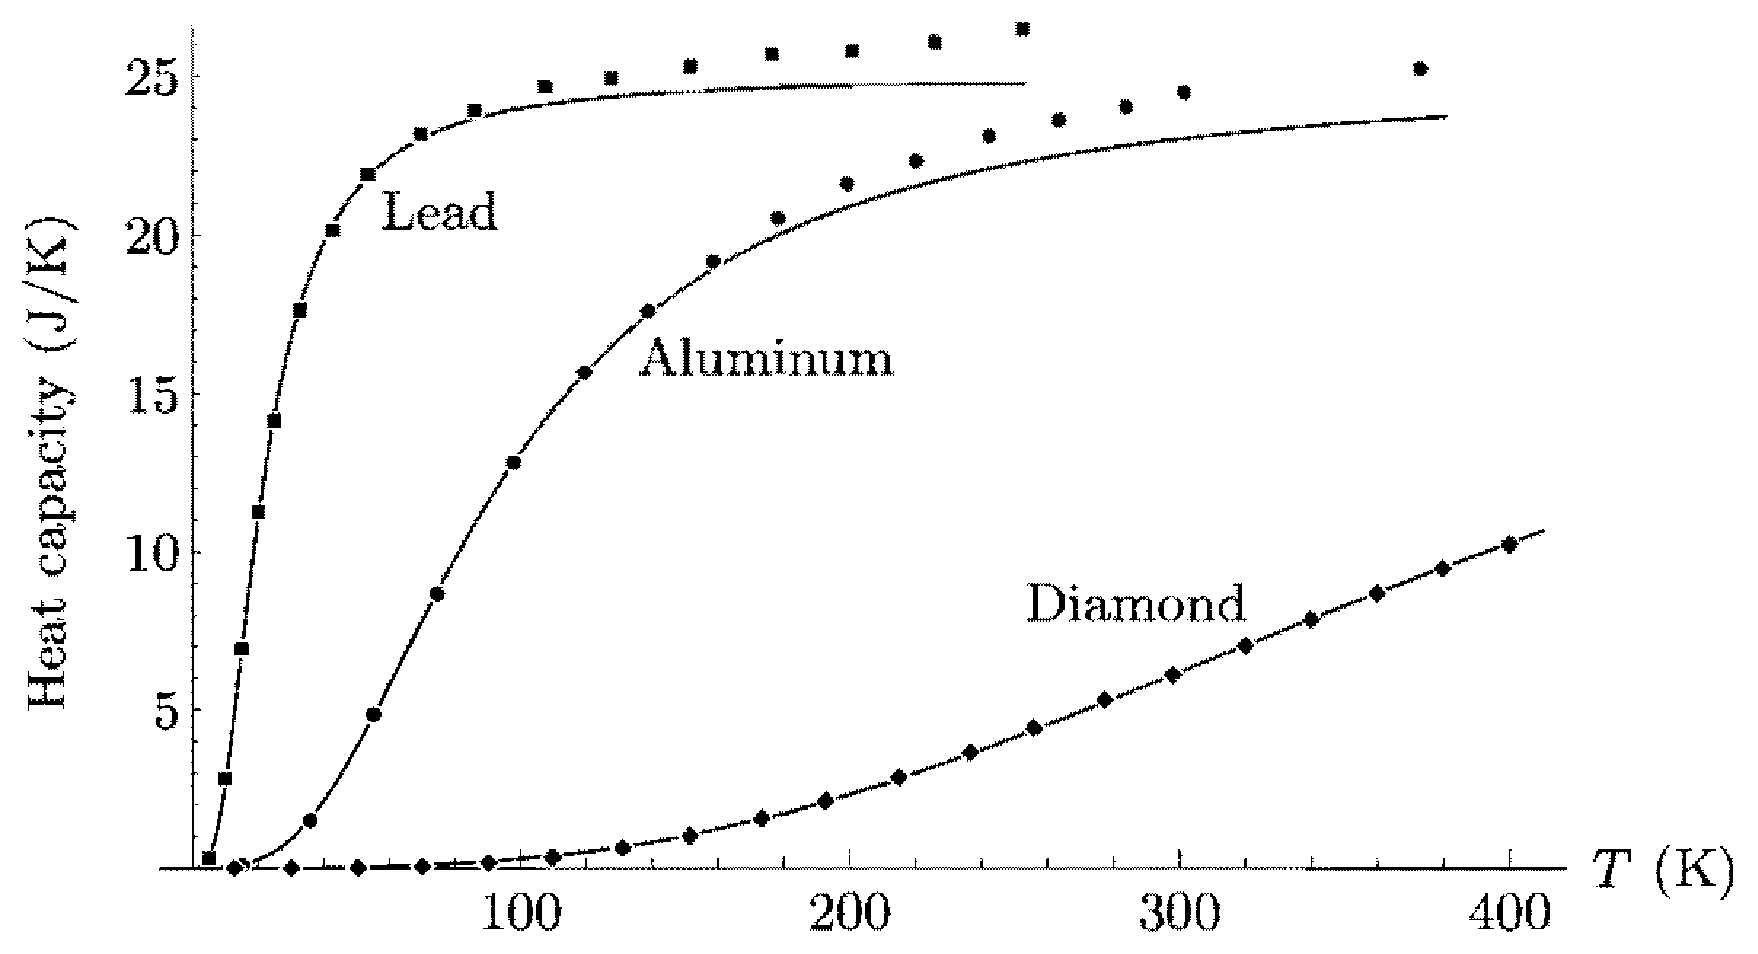
\includegraphics[width=0.7\textwidth]{figs/heat_cap.pdf}\end{center}

Recalling $c_v = \pderiv{E}{T}$, you should have no trouble convincing yourself that the classical non-relativistic ideal gas provides a poor model.
A potentially more promising system could be the $N$ distinguishable spins in a solid we analysed in late February (Section~3.4 of the lecture notes).
We found that this system has internal energy $E = -NH\tanh(\be H)$ for inverse temperature $\be = 1 / T$ and magnetic field strength $H$.
What is the corresponding heat capacity?
How does it compare to the figure above?

You should find poor agreement --- especially upon turning off the external field by taking $H \to 0$!
Physicists in the 1800s also struggled to explain the temperature dependence of experimentally measured heat capacities.
To address this problem, in 1907 Einstein developed a simple model of solids based on quantized energies, taking some inspiration from his famous 1905 proposal that quantized energies explain the \href{https://en.wikipedia.org/wiki/Photoelectric_effect}{photoelectric effect}.

The `Einstein solid' consists of many atoms whose positions are fixed to (distinguishable) locations in a regular lattice.
Interactions between neighbouring atoms are credited with pinning each atom to its fixed location.
This is modeled by picturing neighbouring atoms connected by `oscillators', analogous to springs, which possess energy as a consequence of these interactions.
We define the Einstein solid by hypothesizing that the energy of each oscillator is quantized, $\eps_i = 0, \hbar \om$, $2\hbar \om$, $\cdots$, with the same characteristic angular frequency \om for all oscillators.
Although the oscillators model interactions between nearest-neighbour atoms, in this approach they are \textit{non-interacting} degrees of freedom that we can analyse using tools we have already developed.

As illustrated by the figure below, also from Schroeder's \textit{Introduction to Thermal Physics}, the number of oscillators depends both on the number of atoms and their layout.
In this two-dimensional square lattice, $N$ oscillators would correspond to $N / 2$ atoms in the solid.
In a three-dimensional simple cubic lattice, $N$ oscillators would correspond to $N / 3$ atoms. \\[-24 pt]
\begin{center}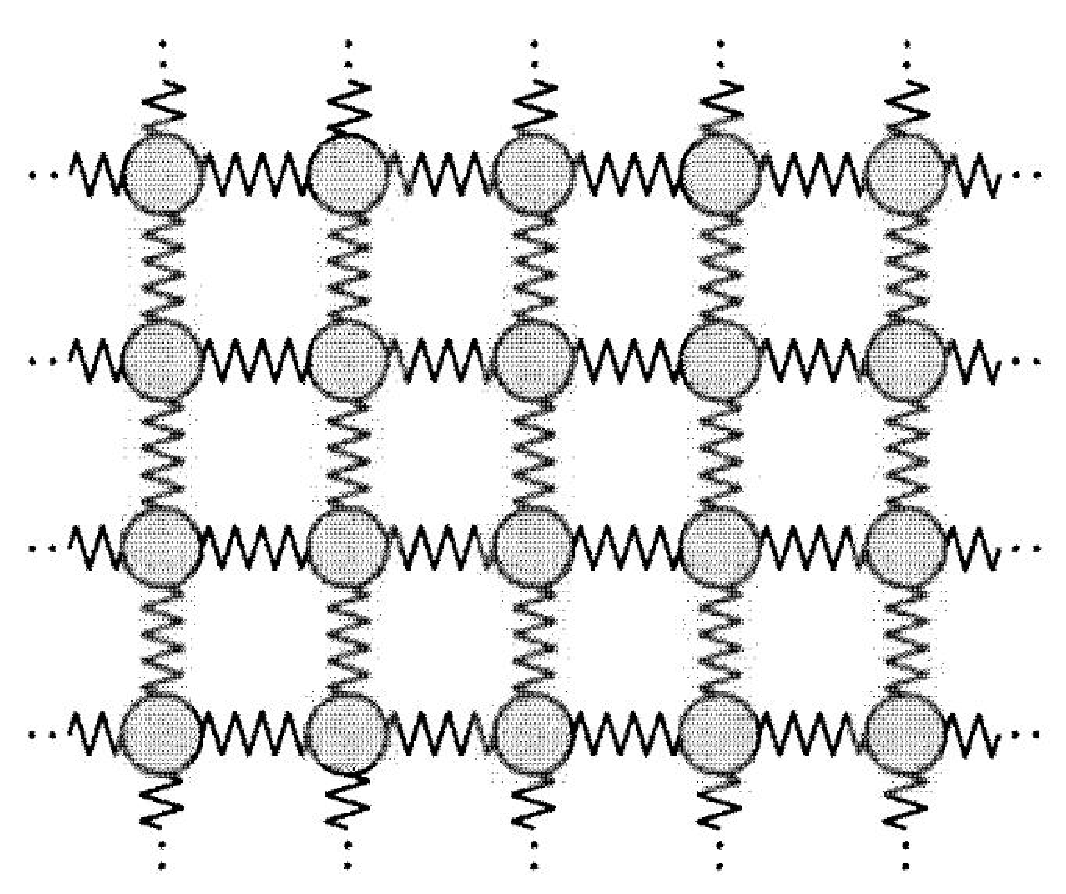
\includegraphics[width=0.4\textwidth]{figs/solid.pdf}\end{center}

The task is to compute the heat capacity for an Einstein solid.
Let's begin by working in terms of the micro-canonical ensemble, fixing the total energy
\begin{equation*}
  E = \sum_i \eps_i = \sum_i k_i\hbar\om \equiv K\hbar\om
\end{equation*}
where $K \equiv \sum_i k_i$ is the integer number of energy `units' available to be distributed among the $N$ oscillators.
Each different way of distributing these $K$ units of energy among the $N$ (distinguishable) oscillators defines a unique micro-state. \\[-24 pt]
\begin{itemize}
  \item What is the total number of micro-states in terms of $N$ and $K$?
        Check your result for a minimal three-oscillator system when it has $K = 0$, $1$, $2$ or $3$ units of energy.

  \item Now consider $K \gg 1$ and $N \gg 1$, so that we can apply Stirling's formula while also approximating $N - 1 \approx N$ and $K - 1 \approx K$.
        What is the resulting entropy?

  \item What is the temperature $T(E)$ of the Einstein solid?
        Is it a `natural' system with non-negative temperature?
\end{itemize}

Now let's change perspective to work in terms of the canonical ensemble, by inverting $T(E)$ to find the internal energy expectation value in terms of the temperature.
Differentiating this $\vev{E}\!(T)$ provides the heat capacity $c_v$ for the Einstein solid.
What is $c_v$ in terms of $x \equiv \hbar \om / T$?
How does it compare to the figure above?
In particular, what are the leading corrections to the high- and low-temperature limits of $c_v$?

While the Einstein solid describes the experimental data much better than the non-interacting spins we first considered, there is still room for improvement\dots

\end{document}
% ------------------------------------------------------------------
